\documentclass[18 pt]{beamer}
\usetheme{Madrid}
% \usefonttheme{professionalfonts}
\usefonttheme{structurebold}
\usecolortheme{rose}
\setbeamerfont{title}{size=\LARGE, series=\bfseries}
\title{Synthesis on Atom Computation}


\usepackage{amsmath}
\usepackage{amssymb}
\usepackage{listings}
\usepackage{booktabs}
\usepackage{multirow}
\usepackage{multirow}
\usepackage{lmodern}
\usepackage{xcolor}
\usepackage{float}
\lstset{
  language=Python,  %代码语言使用的是matlab
  % frame=shadowbox, %把代码用带有阴影的框圈起来
  rulesepcolor=\color{red!20!green!20!blue!20},%代码块边框为淡青色
  keywordstyle=\color{blue!90}\bfseries, %代码关键字的颜色为蓝色,粗体
  commentstyle=\color{red!10!green!70}\textit,    % 设置代码注释的颜色
  basicstyle=\footnotesize,
  showstringspaces=true,%不显示代码字符串中间的空格标记
  % numbers=left, % 显示行号
  % numberstyle=8pt,    % 行号字体
  % numberstyle=\color{green},
  stringstyle=\rmfamily\slshape\color[RGB]{128,0,0}, % 代码字符串的特殊格式
  breaklines=true, %对过长的代码自动换行
  extendedchars=false,  %解决代码跨页时,章节标题,页眉等汉字不显示的问题
  escapeinside=``,%代码中出现中文必须加上,否则报错
  texcl=true}

\lstset{breaklines}%自动将长的代码行换行排版

\lstset{extendedchars=false}%解决代码跨页时,章节标题,页眉等汉字不显示的问题

\usepackage{textcomp}
% \usepackage[margin=1in]{geometry}
\usepackage{pythonhighlight}
% \usepackage{minted}
\usepackage[backend=bibtex]{biblatex}
%\usepackage[style=authortitle,backend=biber]{biblatex}
\addbibresource{ResearchRabbit_Export_2022_10_20.bib}

\usepackage{algorithm}
\usepackage{algorithmic}
\renewcommand{\algorithmicrequire}{\textbf{Input:}}
\renewcommand{\algorithmicensure}{\textbf{Output:}}


\setbeamertemplate{footline}[frame number]
\begin{document}
\begin{frame}[plain]
    \titlepage
\end{frame}
\section{Compilation for Dynamically Field-Programmable Qubit Arrays with Efficient and Provably Near-Optimal Scheduling}
\begin{frame}
    \frametitle{Related Works}
    \begin{itemize}
        \item \textbf{\textit{Compiling Quantum Circuits for Dynamically Field-Programmable Neutral Atoms Array Processors}}: Utilizes Z3 MST, but lacks scalability and fidelity considerations.
        \item \textbf{\textit{FPQA-C: A Compilation Framework for Field Programmable Qubit Array}}: Employs a rule-based algorithm, offering good scalability, but does not achieve the optimal count of 2Q gates.
    \end{itemize}
    \begin{figure}
        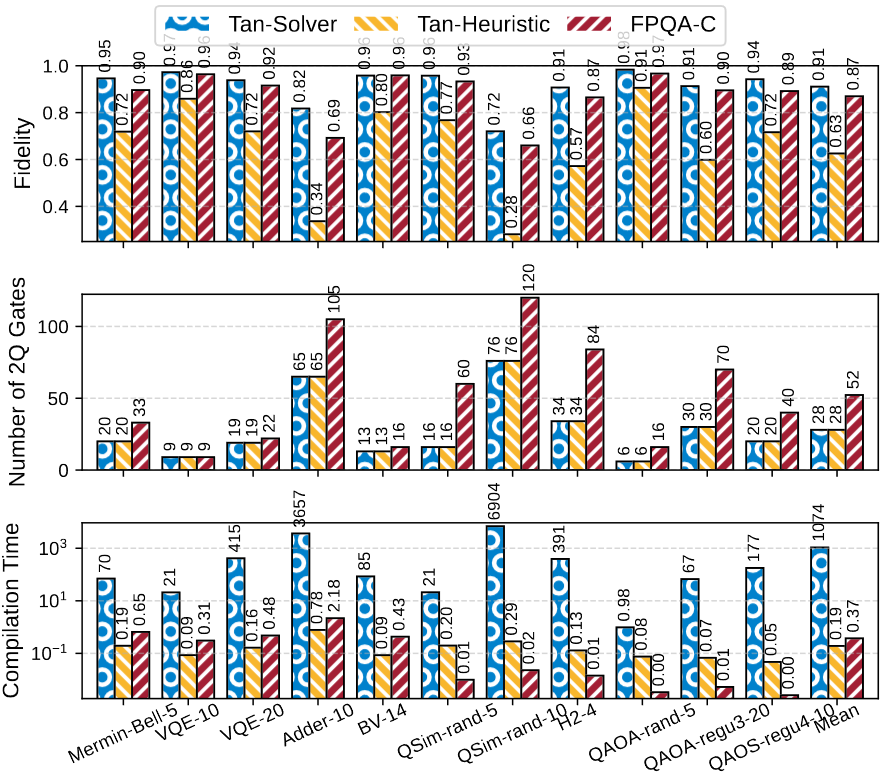
\includegraphics[height=5cm]{back.png}
    \end{figure}
\end{frame}

\begin{frame}
    \frametitle{Overview}
    \begin{itemize}
        \item Background: Quantum computing with neutral atoms has advanced rapidly.
        \item Fidelity: \(f=\left(f_{1}\right)^{g_{1}} \cdot \overbrace{\left(f_{2}\right)^{g_{2}} \cdot\left(f_{\text {exc }}\right)^{|Q| S-2 g_{2}}}^{\text {two-qubit gate }} \cdot \overbrace{\left(f_{\text {trans }}\right)^{N_{\text {trans }}}}^{\text {atom transfer }}\cdot \overbrace{\prod_{q\in Q} (1-T_q/T_2)}^{decoherence}\).
        \item Significant scalability: experiments with up to 6,100 qubits.
        % \item Challenges in fully leveraging hardware flexibility while respecting constraints.
        \item The compilation process is broken down into three tasks: scheduling, placement, and routing.
    \end{itemize}
\end{frame}

\begin{frame}
    \frametitle{Scheduling}
    \begin{itemize}
        \item Scheduling is crucial for determining the sequence of operations.
        \item The approach uses graph edge coloring for optimal scheduling.
        \item Ensures near-optimal stage count for two-qubit gates.
        \item Proven to be at most one stage more than the optimal solution.
        \item This reduces the fidelity bottleneck in this platform.
    \end{itemize}
\end{frame}

\begin{frame}
    \frametitle{Scheduling: Graph Edge Coloring}
    \begin{itemize}
        \item Graph edge coloring is used to model the scheduling problem.
        \item Each edge represents a two-qubit gate.
        \item Colors represent different stages.
        \item The goal is to minimize the number of stages while ensuring no two adjacent edges share the same color.
    \end{itemize}
\end{frame}

\begin{frame}
    \frametitle{Placement}
    \begin{itemize}
        \item Placement refers to assigning qubits to physical locations.
        \item Optimal placement minimizes the distance between interacting qubits.
        \item This reduces the need for long-distance routing, which can lower fidelity.
        \item Placement strategies must handle large qubit arrays efficiently.
    \end{itemize}
\end{frame}

\begin{frame}
    \frametitle{Placement Strategies}
    \begin{itemize}
        \item Use of heuristic algorithms to find near-optimal solutions.
        \item Consideration of hardware constraints and qubit connectivity.
        \item Balancing between computational efficiency and placement quality.
    \end{itemize}
\end{frame}

\begin{frame}
    \frametitle{Routing}
    \begin{itemize}
        \item Routing involves determining paths for qubits to move during computation.
        \item Efficient routing algorithms are essential to maintain high fidelity.
        \item Routing must handle constraints such as limited movement and interaction range.
        \item Ensuring minimal delay and avoiding congestion are key goals.
    \end{itemize}
\end{frame}

\begin{frame}
    \frametitle{Routing Algorithms}
    \begin{itemize}
        \item Use of shortest path algorithms to determine efficient routes.
        \item Dynamic adaptation to changing qubit positions and interactions.
        \item Balancing the trade-off between routing efficiency and computational overhead.
    \end{itemize}
\end{frame}

\begin{frame}
    \frametitle{Results and Comparison}
    \begin{itemize}
        \item The compiler, Enola, shows significant improvements in performance.
        \item Achieves 3.7X stage reduction compared to existing works.
        \item Demonstrates 5.9X improvement in fidelity on benchmark sets.
        \item Highly scalable, capable of compiling circuits with up to 10,000 qubits within 30 minutes.
        \item Outperforms the current state of the art, OLSQ-DPQA.
    \end{itemize}
\end{frame}

\begin{frame}
    \frametitle{Performance Metrics}
    \begin{itemize}
        \item Stage count reduction: Enola vs. OLSQ-DPQA.
        \item Fidelity improvement: Quantitative comparisons.
        \item Scalability: Handling large-scale quantum circuits efficiently.
    \end{itemize}
\end{frame}

\begin{frame}
    \frametitle{Conclusion}
    \begin{itemize}
        \item The compilation process for dynamically field-programmable qubit arrays involves scheduling, placement, and routing.
        \item The method provide near-optimal solutions for scheduling and efficient strategies for placement and routing.
        \item Enola compiler achieves significant improvements in stage reduction and fidelity.
        \item Future work includes further optimization and exploring additional constraints.
        \item Open source availability: \url{https://github.com/UCLA-VAST/Enola}
    \end{itemize}
\end{frame}
\end{document}
